\documentclass{beamer}
\usepackage{tikz}
\usepackage{hyperref}
\usepackage{listings}
\usepackage{xcolor}

\definecolor{codegreen}{rgb}{0,0.6,0}
\definecolor{codegray}{rgb}{0.5,0.5,0.5}
\definecolor{codepurple}{rgb}{0.58,0,0.82}
\definecolor{backcolour}{rgb}{0.95,0.95,0.92}

\lstdefinestyle{mystyle}{
    backgroundcolor=\color{backcolour},   
    commentstyle=\color{codegreen},
    keywordstyle=\color{magenta},
    numberstyle=\tiny\color{codegray},
    stringstyle=\color{codepurple},
    basicstyle=\ttfamily\footnotesize,
    breakatwhitespace=false,         
    breaklines=true,                 
    captionpos=b,                    
    keepspaces=true,                 
    numbers=left,                    
    numbersep=5pt,                  
    showspaces=false,                
    showstringspaces=false,
    showtabs=false,                  
    tabsize=2,
    escapeinside={\%*}{*)}
}

\lstset{style=mystyle}

\title{Campus Network Design and Implementation}
\subtitle{Computer Network-1 Course Project}
\author{Theodoros}
\institute{Contributors: }
\begin{document}

\frame{\titlepage}

\begin{frame}
\frametitle{Contents}
\tableofcontents
\end{frame}

\section{Network Design}
\begin{frame}
\frametitle{Network Design}
\begin{itemize}
    \item \hyperlink{design}{1. Network Design}
    \item \hyperlink{config}{2. Network Configuration}
    \item \hyperlink{routing}{3. Static/Dynamic Routing} (To be added)
    \item \hyperlink{dhcp}{4. DHCP Configuration} (To be added)
    \item \hyperlink{vlans}{5. VLAN Configuration} (To be added)
    \item \hyperlink{testing}{6. Network Testing} (To be added)
\end{itemize}
\end{frame}

\begin{frame}[label=design]
\frametitle{Network Diagram}
\begin{center}
\resizebox{0.85\textwidth}{!}{
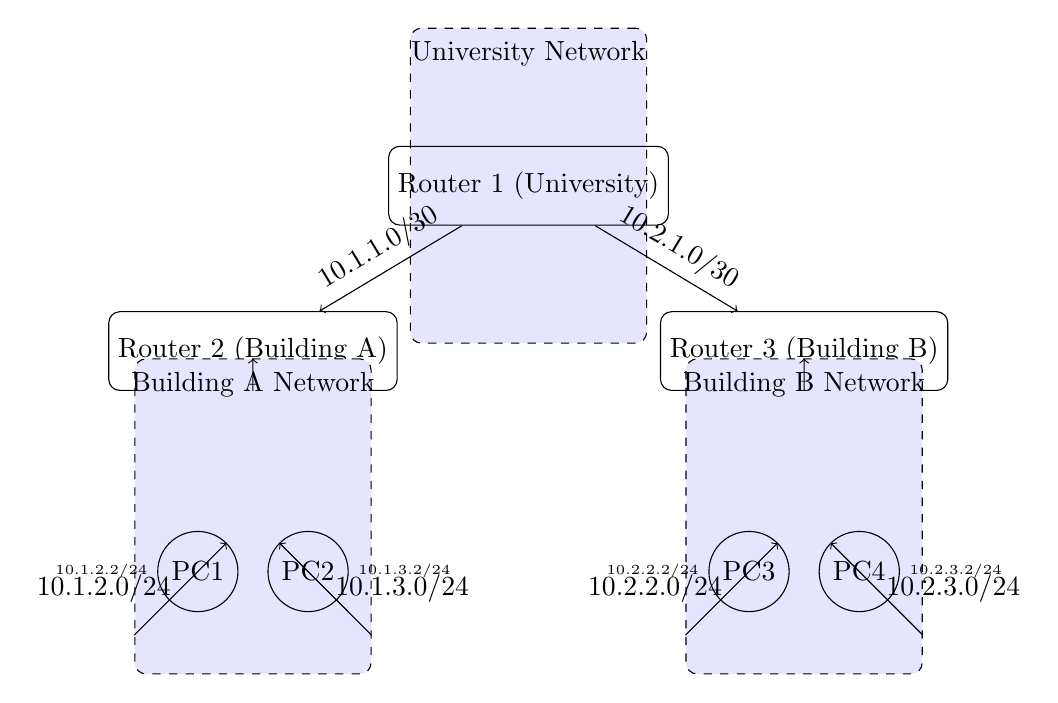
\begin{tikzpicture}[scale=0.7]
    % Define router shapes
    \tikzstyle{router}=[draw, rectangle, rounded corners, minimum width=2cm, minimum height=1cm]
    \tikzstyle{pc}=[draw, circle, minimum width=1cm]
    \tikzstyle{network}=[draw, dashed, rectangle, rounded corners, minimum width=3cm, minimum height=4cm, fill=blue!10]
    
    % Place university network
    \node[network] (uni_network) at (0,0) {};
    \node[above] at (0,2) {University Network};
    
    % Place routers
    \node[router] (r1) at (0,0) {Router 1 (University)};
    \node[router] (r2) at (-5,-3) {Router 2 (Building A)};
    \node[router] (r3) at (5,-3) {Router 3 (Building B)};
    
    % Place Building A network
    \node[network] (bldgA) at (-5,-6) {};
    \node[above] at (-5,-4) {Building A Network};
    
    % Place Building B network
    \node[network] (bldgB) at (5,-6) {};
    \node[above] at (5,-4) {Building B Network};
    
    % Place PCs
    \node[pc] (pc1) at (-6,-7) {PC1};
    \node[pc] (pc2) at (-4,-7) {PC2};
    \node[pc] (pc3) at (4,-7) {PC3};
    \node[pc] (pc4) at (6,-7) {PC4};
    
    % Connect routers
    \draw[->] (r1) -- node[above, sloped] {10.1.1.0/30} (r2);
    \draw[->] (r1) -- node[above, sloped] {10.2.1.0/30} (r3);
    
    % Connect PCs to routers
    \draw[->] (r2) -- (bldgA);
    \draw[->] (r3) -- (bldgB);
    \draw[->] (bldgA) -- node[left] {10.1.2.0/24} (pc1);
    \draw[->] (bldgA) -- node[right] {10.1.3.0/24} (pc2);
    \draw[->] (bldgB) -- node[left] {10.2.2.0/24} (pc3);
    \draw[->] (bldgB) -- node[right] {10.2.3.0/24} (pc4);
    
    % IP Address labels
    \node[left, font=\tiny] at (pc1.west) {10.1.2.2/24};
    \node[right, font=\tiny] at (pc2.east) {10.1.3.2/24};
    \node[left, font=\tiny] at (pc3.west) {10.2.2.2/24};
    \node[right, font=\tiny] at (pc4.east) {10.2.3.2/24};
\end{tikzpicture}
}
\end{center}
\end{frame}

\begin{frame}[label=config]
\frametitle{Network Configuration}
\begin{itemize}
    \item The network is configured using MikroTik RouterOS commands
    \item Each router has a unique identity and IP addressing scheme
    \item PCs are configured with static IP addresses and default gateways
    \item The network follows a hierarchical design with:
    \begin{itemize}
        \item 10.1.x.x for Building A networks
        \item 10.2.x.x for Building B networks
    \end{itemize}
\end{itemize}
\end{frame}

\begin{frame}
\frametitle{Router Configuration: University Router (R1)}
\begin{lstlisting}[escapechar=|]
# Set router identity
system identity set name="university"

# Configure interfaces
ip address add address=10.1.1.1/30 interface=ether1
ip address add address=10.2.1.1/30 interface=ether2
\end{lstlisting}

\begin{table}
\centering
\begin{tabular}{|l|l|l|}
\hline
\textbf{Address} & \textbf{Network} & \textbf{Interface} \\
\hline
10.1.1.1/30 & 10.1.1.0 & ether1 \\
\hline
10.2.1.1/30 & 10.2.1.0 & ether2 \\
\hline
\end{tabular}
\end{table}

\textbf{Explanation:} 
\begin{itemize}
    \item The central university router connects to Building A and B routers
    \item Point-to-point links use /30 subnets (2 usable addresses)
\end{itemize}
\end{frame}

\begin{frame}
\frametitle{Router Configuration: Building A Router (R2)}
\begin{lstlisting}[escapechar=|]
# Set router identity
system identity set name="Building_A"

# Configure interfaces
ip address add address=10.1.1.2/30 interface=ether1
ip address add address=10.1.2.1/24 interface=ether2 
ip address add address=10.1.3.1/24 interface=ether3
\end{lstlisting}

\begin{table}
\centering
\begin{tabular}{|l|l|l|}
\hline
\textbf{Address} & \textbf{Network} & \textbf{Interface} \\
\hline
10.1.1.2/30 & 10.1.1.0 & ether1 \\
\hline
10.1.2.1/24 & 10.1.2.0 & ether2 \\
\hline
10.1.3.1/24 & 10.1.3.0 & ether3 \\
\hline
\end{tabular}
\end{table}

\textbf{Explanation:}
\begin{itemize}
    \item ether1: Uplink to University Router
    \item ether2: First LAN subnet for PC1
    \item ether3: Second LAN subnet for PC2
\end{itemize}
\end{frame}

\begin{frame}
\frametitle{Router Configuration: Building B Router (R3)}
\begin{lstlisting}[escapechar=|]
# Set router identity
system identity set name="Building_B"

# Configure interfaces
ip address add address=10.2.1.2/30 interface=ether1
ip address add address=10.2.2.1/24 interface=ether2    
ip address add address=10.2.3.1/24 interface=ether3
\end{lstlisting}

\begin{table}
\centering
\begin{tabular}{|l|l|l|}
\hline
\textbf{Address} & \textbf{Network} & \textbf{Interface} \\
\hline
10.2.1.2/30 & 10.2.1.0 & ether1 \\
\hline
10.2.2.1/24 & 10.2.2.0 & ether2 \\
\hline
10.2.3.1/24 & 10.2.3.0 & ether3 \\
\hline
\end{tabular}
\end{table}

\textbf{Explanation:}
\begin{itemize}
    \item ether1: Uplink to University Router
    \item ether2: First LAN subnet for PC3
    \item ether3: Second LAN subnet for PC4
\end{itemize}
\end{frame}

\begin{frame}
\frametitle{PC Configuration: Building A}
\begin{lstlisting}[escapechar=|]
# PC1 Configuration
PC1> ip 10.1.2.2/24 10.1.2.1
Checking for duplicate address...
PC1 : 10.1.2.2 255.255.255.0 gateway 10.1.2.1

# Test connectivity
PC1> ping 10.1.2.1
84 bytes from 10.1.2.1 icmp_seq=1 ttl=64 time=0.245 ms
84 bytes from 10.1.2.1 icmp_seq=2 ttl=64 time=0.303 ms
...

# PC2 Configuration
PC2> ip 10.1.3.2/24 10.1.3.1
Checking for duplicate address...
PC2 : 10.1.3.2 255.255.255.0 gateway 10.1.3.1

# Test connectivity
PC2> ping 10.1.3.1
84 bytes from 10.1.3.1 icmp_seq=1 ttl=64 time=0.222 ms
...
\end{lstlisting}

\textbf{Explanation:}
\begin{itemize}
    \item Each PC is configured with a static IP and gateway
    \item Basic connectivity test confirms links are active
\end{itemize}
\end{frame}

\begin{frame}
\frametitle{PC Configuration: Building B}
\begin{lstlisting}[escapechar=|]
# PC3 Configuration
PC3> ip 10.2.2.2/24 10.2.2.1
Checking for duplicate address...
PC3 : 10.2.2.2 255.255.255.0 gateway 10.2.2.1

# Test connectivity
PC3> ping 10.2.2.1
84 bytes from 10.2.2.1 icmp_seq=1 ttl=64 time=0.187 ms
...

# PC4 Configuration
PC4> ip 10.2.3.2/24 10.2.3.1
Checking for duplicate address...
PC4 : 10.2.3.2 255.255.255.0 gateway 10.2.3.1

# Test connectivity
PC4> ping 10.2.3.1
84 bytes from 10.2.3.1 icmp_seq=1 ttl=64 time=0.211 ms
84 bytes from 10.2.3.1 icmp_seq=2 ttl=64 time=0.510 ms
84 bytes from 10.2.3.1 icmp_seq=3 ttl=64 time=0.625 ms
\end{lstlisting}

\textbf{Explanation:}
\begin{itemize}
    \item PC3 and PC4 are configured in their respective subnets
    \item Ping tests confirm connectivity to their respective gateways
    \item All PCs are properly configured with the correct IP settings
\end{itemize}
\end{frame}

\section{Next Steps}
\begin{frame}[label=routing]
\frametitle{Static/Dynamic Routing}
% This section will be added later
\end{frame}

\begin{frame}[label=dhcp]
\frametitle{DHCP Configuration}
% This section will be added later
\end{frame}

\begin{frame}[label=vlans]
\frametitle{VLAN Configuration}
% This section will be added later
\end{frame}

\begin{frame}[label=testing]
\frametitle{Network Testing}
% This section will be added later
\end{frame}

\begin{frame}
\frametitle{Conclusion}
\begin{itemize}
    \item \textbf{Current Progress:}
    \begin{itemize}
        \item Network design has been completed
        \item Basic configuration implemented
        \item Local connectivity established
    \end{itemize}
    \item \textbf{Next Steps:}
    \begin{itemize}
        \item Configure routing between subnets
        \item Set up DHCP for automatic IP assignment
        \item Configure VLANs for network segmentation
        \item Test full network connectivity
    \end{itemize}
\end{itemize}
\end{frame}

\end{document}